% !TeX encoding = UTF-8
\chapter{Task 4: Machine Learning Classifiers}\label{chap:task4_ml}

\section{Setup}\label{sec:ml-setup}

We train Logistic Regression (LR, \texttt{max\_iter=5000}) and a Decision Tree (DT, \texttt{random\_state=42}, unpruned) with scikit-learn~\cite{pedregosa2011sklearn}. Each is trained in two variants, default and \texttt{class\_weight="balanced"}. The file has only one attack class, so a multiclass target would duplicate the binary one (BENIGN vs.\ DDoS), and we train four binary models. Every model is one scikit-learn \texttt{Pipeline}: \texttt{MinMaxScaler(clip=True)}, \texttt{SelectKBest(chi2, k=20)} and the classifier (Listing~\ref{lst:pipe}). Scaler and selector are fitted on the training split only (156,157 flows). All models are evaluated on the held-out test split of 66,925 flows, of which 38,404 are DDoS. Inference time is the median of five timed \texttt{predict} calls on the whole test split after one warm-up call, scaled to 1,000 flows. Both LR models converged after 48 iterations, far below the limit of 5,000.

\lstinputlisting[style=py,float=htbp,linerange={22-27,30-38},caption={\texttt{build\_pipeline()} and \texttt{make\_classifier()} in \texttt{src/ddosids/models.py}},label={lst:pipe}]{../src/ddosids/models.py}

\section{Results}\label{sec:ml-binary}

The default DT makes only 7 false positives and 25 false negatives on 66,925 test flows (Table~\ref{tab:t4binary}), which gives a DDoS precision of 0.9998, a recall of 0.9993 and an F1 of 0.9996. Logistic Regression detects almost as many attacks (recall 0.9988, 45 missed flows) but raises about 2,000 false alarms (2,008 for the default and 1,974 for the balanced variant), so its DDoS precision is only about 0.95 and its F1 0.974. Figure~\ref{fig:cm} shows the confusion matrices of the default DT and the balanced LR, and Figure~\ref{fig:ss33} the console output for the default DT.

Class weighting changes almost nothing. For the DT, the balanced variant has exactly the same confusion matrix and metrics as the default one, and for LR the false positives drop only from 2,008 to 1,974. The two classes are close to balanced (57\,\% DDoS and 43\,\% BENIGN after cleaning), so \texttt{class\_weight="balanced"} gives both classes weights close to one. The fit and inference times come from a single run each.

\begin{table}[ht]
	\centering\small
	\resizebox{\linewidth}{!}{% AUTO-GENERATED by scripts/make_report_tables.py from outputs/task4/comparison.csv, outputs/task4/metrics.json -- do not edit
\begin{tabular}{lrrrrrrrrr}
\toprule
Model & Acc. & Macro-F1 & Prec. & Rec. & F1 & FP & FN & Fit (s) & Inf. (ms/1k) \\
\midrule
LR default & 0.9693 & 0.9683 & 0.9503 & 0.9988 & 0.9739 & 2\,008 & 45 & 6.45 & 0.717 \\
LR balanced & 0.9698 & 0.9689 & 0.9511 & 0.9988 & 0.9744 & 1\,974 & 45 & 5.97 & 1.996 \\
\textbf{DT default} & \textbf{0.9995} & \textbf{0.9995} & \textbf{0.9998} & \textbf{0.9993} & \textbf{0.9996} & \textbf{7} & \textbf{25} & \textbf{2.20} & \textbf{0.695} \\
DT balanced & 0.9995 & 0.9995 & 0.9998 & 0.9993 & 0.9996 & 7 & 25 & 1.25 & 0.717 \\
\bottomrule
\end{tabular}
}
	\caption{Binary results on the test split (Prec., Rec., F1 refer to the DDoS class; Macro-F1 averages both classes; FP/FN are false positives and false negatives). Best model in bold.}
	\label{tab:t4binary}
\end{table}

\begin{figure}[htb]
	\centering
	\begin{subfigure}[t]{0.48\linewidth}
		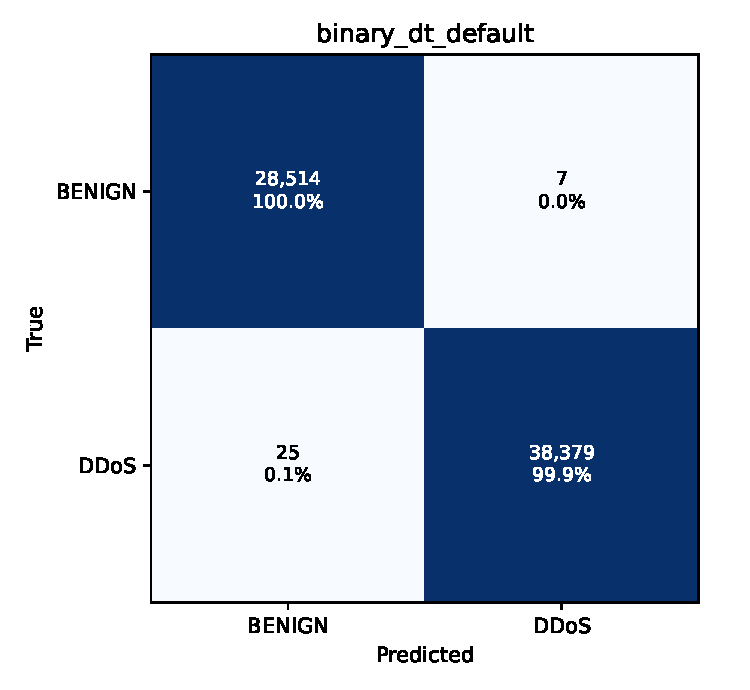
\includegraphics[width=\linewidth]{cm_binary_dt_default.pdf}
		\caption{Decision Tree (default): 7 false positives, 25 false negatives.}
	\end{subfigure}\hfill
	\begin{subfigure}[t]{0.48\linewidth}
		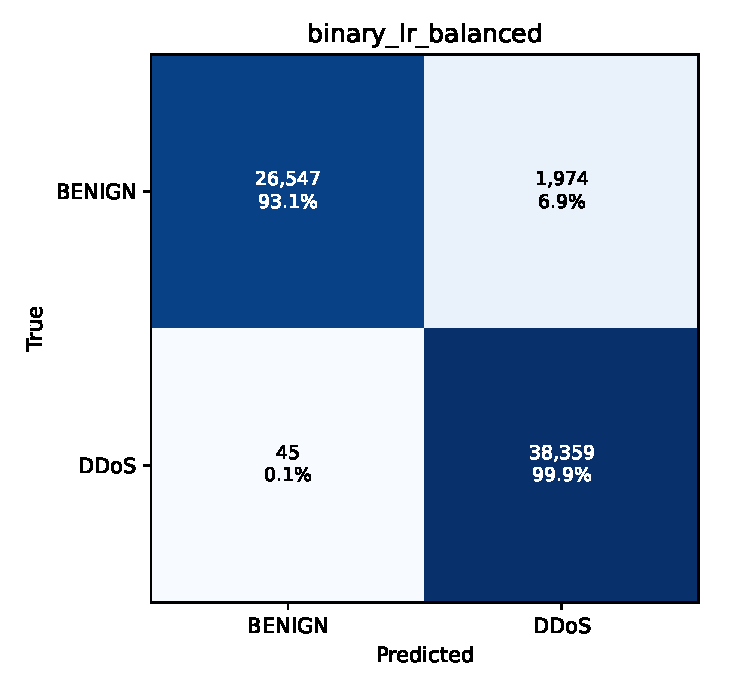
\includegraphics[width=\linewidth]{cm_binary_lr_balanced.pdf}
		\caption{Logistic Regression (balanced): 1,974 false positives, 45 false negatives.}
	\end{subfigure}
	\caption{Confusion matrices of two of the four models (test split).}
	\label{fig:cm}
\end{figure}

\ssfig[0.55\linewidth]{SS33}{Console output of the training script for the chosen model, \texttt{binary\_dt\_default}: per-class report, confusion matrix, and fit and inference times.}{fig:ss33}

\ssfig{SS35}{Comparison table of the four models, as printed by the training script (cf.\ Table~\ref{tab:t4binary}).}{fig:ss35}

\section{Interpretation}\label{sec:ml-interp}

The Decision Tree beats Logistic Regression in every metric of Table~\ref{tab:t4binary}: the DDoS F1 is 0.9996 against at most 0.9744. Attacks occupy narrow value ranges of a few features (packet lengths, port 80, flag counts), and a tree isolates such ranges with axis-aligned thresholds. LR draws a single linear boundary through heavy-tailed, min-max-compressed features and cannot separate the classes as sharply.

We use \texttt{binary\_dt\_default} in the real-time part. Default and balanced DT are identical on the test split, so we take the simpler default model, and it has the fewest errors of all four models. \texttt{Destination Port} is the second-best feature by $\chi^2$ (Table~\ref{tab:t3top20}), and virtually all DDoS flows target port 80, so the near-perfect scores may partly rest on the port as a shortcut (Chapter~\ref{chap:discussion}). Because the test split comes from the same capture as the training data, Chapter~\ref{chap:task4_realtime} also checks the model on traffic from a different network.

\FloatBarrier
